\documentclass[12pt, a4paper]{article}

\usepackage{mmap}
\usepackage[utf8]{inputenc}
\usepackage[english]{babel}
\usepackage{graphicx}
\graphicspath{{Images/}}
\usepackage{amsmath}
\usepackage{amssymb} %specially for circledash (convolution)
\usepackage{systeme} %to make systems of equations with that {
\usepackage{bm} %bold math

\usepackage[shortlabels]{enumitem} %for enumerates with letters \begin{enumerate}[a)] or (a) or others.




\usepackage{geometry} %to change page dimensions
 \geometry{
 a4paper,
 total={170mm,257mm},
 left=20mm,
 top=20mm,
 }



\usepackage{subcaption}
\usepackage{indentfirst}


\usepackage{listings}
\lstset{basicstyle=\ttfamily,columns=flexible}

\usepackage[hidelinks]{hyperref}
\hypersetup{
    linktoc=all,     %set to all if you want both sections and subsections linked
}


\usepackage{verbatim}
\usepackage{ulem} %for uline
\usepackage{todonotes} %for \todo

\usepackage{parskip} %so so so important. It makes everything better


\usepackage{textcomp} %for putting low tildes like $\sim$

\usepackage{enumitem} %for changing easily the items in enumerates and itemizes

\usepackage{multicol} %duh, for multi columns. In itemises, for instance.


\usepackage{multirow} %maybe not used, but to merge cells vertically
\usepackage{diagbox} %to make that sweet diagonal line in tables



%for full script matlab listings.
\usepackage{color} %red, green, blue, yellow, cyan, magenta, black, white
\definecolor{mygreen}{RGB}{28,172,0} % color values Red, Green, Blue
\definecolor{mylilas}{RGB}{170,55,241}


\lstset{language=Matlab,%
    %basicstyle=\color{red},
    breaklines=true,%
    morekeywords={matlab2tikz},
    keywordstyle=\color{blue},%
    morekeywords=[2]{1}, keywordstyle=[2]{\color{black}},
    identifierstyle=\color{black},%
    stringstyle=\color{mylilas},
    commentstyle=\color{mygreen},%
    showstringspaces=false,%without this there will be a symbol in the places where there is a space
    numbers=left,%
    numberstyle={\tiny \color{black}},% size of the numbers
    numbersep=9pt, % this defines how far the numbers are from the text
    emph=[1]{for,end,break},emphstyle=[1]\color{red} 
}
\lstset
{
    language=[LaTeX]TeX,
    breaklines=true,
    basicstyle=\tt\scriptsize,
    keywordstyle=\color{blue},
    identifierstyle=\color{magenta},
}

%test for an alternative for lslisting
%\usepackage{lmodern} % for bold teletype font
%\usepackage{minted}

%for extended coefficient form of the matrixes
\makeatletter
\renewcommand*\env@matrix[1][*\c@MaxMatrixCols c]{%
  \hskip -\arraycolsep
  \let\@ifnextchar\new@ifnextchar
  \array{#1}}
\makeatother

%serve only to only number the referenced equations
\usepackage{mathtools}
\mathtoolsset{showonlyrefs}
%it is a good practice to use this and label everything because it becomes much easier to modify the text know that all labels will be safe




\renewcommand\textbullet{\ensuremath{\bullet}} %to prevent itemize warnings about the font...

\DeclareMathOperator*{\argmax}{arg\,max}
\DeclareMathOperator*{\argmin}{arg\,min}
\newcommand{\image}[4]{
	\begin{center}

		\includegraphics[scale = #4]{#1}
    	\captionsetup{type=figure} 
   		\caption{#2}			
        \label{#3}
        
    \end{center}
}
%possible to use: \ifthenelse{\isempty{#1}}{#1}{default value for #1} for optional arguments

\newcommand{\bb}[1]{
	\textbf{#1}
}
 
\newcommand{\ii}[1]{
	\textit{#1}
}

\newcommand{\ul}[1]{
	\underline{#1}
}


\newcommand{\quickimage}[2]{
	\begin{center}
		\includegraphics[scale = #2]{#1}        
    \end{center}
}


\newcommand{\qlink}[2]{
	\href{#1}{\uline{#2}}
}



\title{Signal Processing Overview}

\author{
    João Morais
}

\date{\today}

 
\begin{document}

\maketitle

\begin{abstract}
    If Signal Processing could be described in one sentence it would be ``How to find something impossible to find using an immense amount of mathematics that are not necessary to apply the final result''. Signal Processing in Communications, more specifically, Array Signal Processing by applying some strong logic to the what is received in the sensors can estimate the channel and effectively receive a signal that has been attenuated, interfered by other signals in the same frequency and distorted by the environment and by itself. Now multiply this by the number of users in a multipath environment and it might become possible to imagine the tip of the iceberg. 
\end{abstract}

\newpage
\tableofcontents
\newpage

\section{Intro} \label{sec:intro}


\par What is Space-Time Processing?
\par Simply put, is processing in space and in time. If there is an array of sensors, there is space processing and if contributions to the same signal come at different time instants, is necessary time processing as well to decide what to account as part of the signal.

There are many advantages of using an array of sensors and STP (Space-Time Processing):
\begin{itemize}
    \item Improve Capacity:
    \item Improve Coverage:
    \item Improve Quality:
    \item Reduces Co-channel Interference (CCI):
    \item Enhances Diversity:
    \item Improves Gain:
\end{itemize}
\section{Coherent adding - The Matched filter}
\par Nothing more than adding in a useful way.
\par When a signal comes from a given directions, the sensors in the array will sense different signals in the same time instant. They will also experience different noises. If we know what are we suppose to observe throughout the sensor array for a given signal, we can check if that is what we indeed received. If that is the case, is because that was the transmitted signal.
\par We can do even further enhancements: in a ULA (Uniform Linear Array), the difference of the signal received in adjacent elements is preserved. Therefore, one can some all the signals scaled by the inverse relation between them. For instance, if the first element receives $s_0$ and the second element receives $s_1  = s_0 \times a$ then we can sum them as $s_o + s_1/a$ and we will get double the first signal and we will cancel out the noise!
\par This is know as the Matched Filter.

If one cares to write more precisely:

\todo{steering vector}
%deduction, and matched filter concise w^H = a




%%%%%%%%%%%%%%%%%%%%%%%%%%%%%%%%%%%%%%%%%%%%%%%%%%%


\begin{equation}
    x_i(t) = a(\theta) \beta s(t) e^{-j 2 \pi f_c r_i}
\end{equation}
Where $a(\theta)$ is the gain of the antenna in the direction of the signal, $s(t)$ is the transmitted signal (already not counting with the delay of propagation due to narrowband assumptions), $f_c$ is the central frequency of the signal and $r_i$ being the distance difference in reference with the first element.

\par The M received signals can be written as:

\quickimage{practice2.png}{.7}

\par Now, two cases are worth distinguishing:

\begin{itemize}
    \item For more than one source, the received signal becomes a superposition of various signals (represented for two sources): 

    \quickimage{practice3.png}{.7}

    \item For the same source with multipath, the received signal will be:
    
    \quickimage{practice4.png}{.6}
\end{itemize}


\par Now, accounting all together, we will have something like: 

\quickimage{practice5.png}{.4}

\par Mathematically: $\mathbf{x}(t) = \mathbf{a_1}s_1(t) + \mathbf{a_2}s_2(t) = A \mathbf{s}(t)$, where $\mathbf{s}(t)$ is a column vector with every source and $A$ is the matrix that accounts for how the signals will be received.

\par Thus, converging to the simple following formula. If we take N samples, then we get the expression below.

\quickimage{practice6.png}{.7}

%continue to beamforming...
%%%%%%%%%%%%%%%%%%%%%%%%%%%%%%%%%%%%%%%%%%%%%%%%%%%%%%%%%%%%%%%%%%%%%%%%

\par As we'll see, the matched filter is not the best estimator because it only works perfectly if the is orthogonality between the symbols. If there isn't, multiplying the transpose won't give identity. A better way of processing would be to multiply the inverse and this is what is called a Zero Forcing estimator.




\subsection{Matched Filter vs Zero Forcing vs Wiener Filter}
\par One is said to be perfect for just noise, the other perfect for just ISI and the last seems to find the best result of both. The expressions first:
\todo{ (check these properly)}
\begin{align}
    W^H &= A^H \\
    W^H &= H^\dagger \\
    W &= R_X^{-1}H = (H H^H + \sigma^2I)^{-1}\mathbf{H}
\end{align}

\par The matched filter can deliver results as good as the Zero Forcing if there is no noise. Without noise, the symbols should still be orthogonal and the inverse multiplied by the matrix that is not inverted will give the identity and so will the transposed only because of the orthogonality. 



-c pseudo inverse can make the noise explode, that is why the ZF can make the noise worse. This is related with the condition number. If we simply take the hermitian, the noise can never explode because there is no risk of any element be close to infinity.
This is why MF minimises noise and ZF the interference: ZF focus on really inverting the matrix that will return the identity and make the symbols not interfere with each other by successfully undoing the mixing the channel has just done.

The wiener receiver accounts the noise as well. And tends to one of the other two receivers if the noise or interference are much bigger than the other. If there is too much noise, the wiener optimises it and becomes very close to the MF so that we can have the best compromise between optimisations.




\section{Important math} \label{sec:important_math}

\subsection{Norms} \label{sec:important_math_norms}
\par Basically, there are two or three norms that we should keep in mind. One that applies to vectors and two that apply to matrices.

\quickimage{./web/algebra1.png}{.7}


\quickimage{./web/algebra2.png}{.7}

\subsection{Means and Variances} \label{sec:important_math_variances}

\todo{Finish the review of the final assignment}
\todo{learn about each beamformer principle}

\par The mean is very self-explanatory.
\par The variance is measure of how much and how frequently the signal varies from the mean:

\quickimage{wiki1var.png}{.8}

\par And some important properties about it:

\begin{align}
    & Var(X) \geq 0 \\
    & P(X = a) = 1  \Rightarrow Var(X) = 0 \\
    & Var(X + a) = Var(X) \\
    & Var(aX) = a^2 Var(X)
\end{align}

\par Consider the following example. We have a vector of measurements with 100 elements and 50 of those elements have the value 100 and the other 50 have the value 200.
From applying the variance we we'll see that the variance of this set of measurements is $50^2$, so the standard deviation which is the square root of the variance, will be 50. 
\par What does this mean? Well, the standard deviation is exactly that. However, what is standard is not what is expected. The expected is the mean or the average and they happen to coincide in this fortunate example.
\par Another question: why do we use the standard deviation and not the average deviation? Well, they give different results! The major difference between them is that using $\sqrt{E[(X-\mu^2)]}$ instead of $E[|X-\mu|]$ will give an higher importance to bigger deviation while the latter will give the same important to all. If we think about it: it should be much more likely to be a small deviation, it should be more likely to be close to the mean. Therefore, there should be an importance scaling when we see a bigger deviation because it should be hard to come by so if it appeared, that should be considered. One can see it as a Pythagorean Theorem of statistics.

\subsubsection{Variance = Power? SNR($\sigma$)}
Yes, if the signal has null mean.

The power of a signal can be obtained from: $P(X) = \frac{1}{N}\sum_i=1^Nx_i^2$, the total energy divided by the time intervals/number of samples.

Thus, to include noise in a signal such that it has a certain SNR, we need to calculate the signal power at the reception, lets called it S' since S was the original transmitted signal. Then: $SNR = \frac{S'}{P_N} = \frac{S'}{\sigma_N}$. And don't forget the SNR is in linear units. To obtain the variance the formula ust has to be inverted accordingly.

\subsection{Unitary Matrix, Isometry and Projections}
\par Lacking the time to properly explain, the slides do a excellent job summing it up:

\quickimage{slides9.png}{.55}
\quickimage{slides10.png}{.5}
\quickimage{slides11.png}{.5}
\quickimage{slides12.png}{.55}
\quickimage{slides13.png}{.55}




\subsection{Singular Value Decomposition} \label{sec:important_mat_svd}

\todo{MERGE} %Note you've probably noticed how there is a fundamental sequence for presenting events and topics regarding math in particular and everything else in general. Therefore, what I explained in The Document about basis and all that should come before this. 

%SO: I should unite this with the document, or at least the maths part. But what I should really really do is find a way of being able to write in different documents, or else that document will be to heavy to compile at once. This would also help me to prepare the thesis document.

%until then, it is ok to do everything or the most part here.

\par Once again the slides sum this up perfectly and as such a direct use will be made:

\quickimage{slides14.png}{.55}
\quickimage{slides15.png}{.55}

\par More exactly regarding the end, $\mathbf{\hat{U}}$ will have d column vectors in it and $\mathbf{\hat{V}}^H$ will have d row vectors in it.

\par Now some facts about SVD will introduce perfectly the next section where they are carefully explained.

\quickimage{slides16.png}{.55}

\todo{explain} %the facts not justified in the net sections

\subsection{Matrices Perspectives and Spaces Relations} \label{sec:important_math_spaces_relations}

\par The facts that should have been particularly hard to swallow where the ones related with the basis. These happen to be the easiest to explain!
\par In the intro of a matrix, it is explained the following:

\begin{equation}
    \begin{pmatrix}
        1 & 2 & 3 \\
        6 & 5 & 4 \\
        7 & 8 & 9 
    \end{pmatrix}
    \begin{pmatrix}
        x \\
        y \\
        z
    \end{pmatrix}
    = 
    \begin{pmatrix}
    1 \\
    6 \\
    7    
    \end{pmatrix}x + 
    \begin{pmatrix}
        2 \\
        5 \\
        8
    \end{pmatrix}y + 
    \begin{pmatrix}
        3 \\
        4 \\
        9
    \end{pmatrix}z
\end{equation}

\par Therefore it becomes clear that \uline{the column space of the result will be a subset of the column space of the first matrix, because the column of the result will be a linear combination of those the columns of the first matrix}. For bigger matrices being multiplied on the right, we'll have no more than more columns on the right of the result column. 

\par In fact, the 3 matrix perspectives are:
\begin{itemize}
    \item the first column of the result will be the a linear combination of the columns of B by the entrances along the first column C, exactly like above;
    \item for A = BC : from the above we see that only the first entrances of the columns of B matter for the first entrance of the resulting column, therefore we see that multiplying the first (or the i-th) row of B with the first (or j-th) column of C we get the  entrance (1,1) of A (or (i,j)  $\rightarrow A_{ij}$);
    \item slightly harder to notice is now:
    
\begin{equation*}
    \begin{pmatrix}
        1 & 2 & 3 \\
        6 & 5 & 4 \\
        7 & 8 & 9 \\
        0 & 1 & 1
    \end{pmatrix}
    \begin{pmatrix}
        1 & 2 & 3 \\
         &  &  \\
         &  &  \\
    \end{pmatrix}
    =
\end{equation*}

\begin{equation*}
    \begin{pmatrix}
        1 & 2 & 3
    \end{pmatrix}1 + 
    \begin{pmatrix}
        1 & 2 & 3
    \end{pmatrix}2 + 
    \begin{pmatrix}
        1 & 2 & 3
    \end{pmatrix}3 = 
    \begin{pmatrix}
        6 & 12 & 18 \\
         &  &  \\
         &  &  \\
         &  & 
    \end{pmatrix}
\end{equation*}
        The rows of A will be the linear combination of the rows of C.
\end{itemize}


\par And these 3 perspectives are enough to relate various spaces of each matrix:
\begin{itemize}
    \item The column span of A is a subset of the column span of B;
    \item The row span and the row kernel of A is a subset of the row span and the kernel of C
\end{itemize}


\vspace{.5cm}

\bb{\large But let us take one other approach: Dimensions}

If matrix has full rank, it has a rank that is equal to the smallest dimension.

Having in mind that A belongs in $\Re^{m\times n}$, being m the number of rows and n the number of columns, the following four spaces are going to exist if A is rank deficient.
\begin{itemize}
    \item Column space of A - $C(A)$
    \item Row space of A - $C(A^\text{T})$
    \item Nullspace of A - $N(A)$
    \item Left Nullspace of A - $N(A^\text{T})$
\end{itemize}

\Vhrulefill
\par Note that if A is rank deficient, even if m = n, there will be rows and columns without pivots when we put the matrix in reduced row echelon form. The "free variables", the variables without pivots in them, will belong to the nullspaces such that: 
\begin{itemize}
    \item if $r < m$, the row nullspace, or simply nullspace, will have dimension $m-r$
    \item if $r < n$, the column nullspace, or the left nullspace, will have dimension $n-r$
\end{itemize}
\Vhrulefill

This is more formally known as:
\begin{center}
    \bb{\uline{The Fundamental Theorem of Algebra}}.    
\end{center}








\vspace{1cm}

\par Give the relation presented before, one may go further and explain these:

\quickimage{slides17.png}{.55}

\par Since we can see any pair of matrices as only one:
\begin{itemize}
    \item Because $\mathbf{U}$ and $\mathbf{V}$ are unitary, if they form a basis of a space, that basis will be a orthonormal basis.
    \item Given that we may write $\mathbf{X} = \mathbf{\hat{U} \hat{\Sigma} \hat{V}}^\text{H}$, from what was mentioned before we can see that $\mathbf{\hat{U}}$ columns span the space of the columns of X like $\mathbf{\hat{V}}^\text{H}$ spans the space of the rows of X, or equivalently, $\mathbf{\hat{V}}$ is an orthonormal basis for the space of the columns of $\mathbf{X}^\text{H}$.
    \item Since $\mathbf{\hat{U}}^\perp$ is orthogonal to $\mathbf{\hat{U}}$, it will span an orthogonal space, and the space orthogonal to the columns of $\mathbf{X}$ is the kernel of $\mathbf{X}^\text{H}$, which is the left nullspace or the nullspace of the columns of $\mathbf{\hat{U}}$. Similar with $\mathbf{\hat{V}}$
\end{itemize}


\subsection{SVD geometrical Interpretation}
\par Only for curiosity purposes:

\quickimage{slides18.png}{.5}

\par One can see that the singular vectors are scaled by the singular values, that they are orthogonal to each other and that the singular vectors will span the same space as the vectors in X. Therefore, if there is a linear dependent vector in  X, the number of singular vectors will continue the same, as many as the rank of X. The zeros in the central matrix is what allows the "addition" of the orthogonal matrices, because they will be multiplied to 0. The \ii{economy size} SVD provides only left and right singular vectors such that there are non-zero singular values in the middle matrix.




\subsection{Pseudo-Inverse} \label{sec:important_math_pseudoinverse}
An extremely important topic: can you invert a non-square matrix?
Well, obviously no, but you can do your best approximation of it.

The above sections need a slightly further explanation, but in essence, the idea is fully explained in the following 3 slides:

\quickimage{slides19.png}{.5}
\quickimage{slides20.png}{.5}
\quickimage{slides21.png}{.5}




\subsection{Short and Important considerations}

\begin{itemize}
    \item \uline{The maximum rank is the smallest of the dimensions: if it has more unknowns than equations, the maximum rank is the number of\\ equations. If it has more equations than unknowns, the maximum rank is the number of unknowns};
    \item The Toeplitz structure is having the diagonal entrances, from left to right, top to bottom, equal. Like:
    \quickimage{./web/toeplitz.png}{.6}
\end{itemize}

%%%%%%%%%%%%%%%%%%%%%%%%%%%%%%%%%%%%%%%%%%%%%%%%%%%%%%%%%%%%%%%%%%%
\section{Constant Modulus Algorithm}
Exploring the characteristic that many of our transmitted signals have constant modulus (FM, PH, FSK, PSK...), we can use this property in the estimation, by looking of a weights vector that leads to estimations of modulus 1. 

\quickimage{./cma/1.png}{.55}

\quickimage{./cma/2-1.png}{.5}

As should be expected, the cost function we want to minimise, may very well not be trivial to visualize.

\quickimage{./cma/2-2.png}{.55}

A cost function can simply be the distance of the modulus of our prediction $y_k$ to 1. Since we want to minimise that cost function, we will take little steps in the direction of the minimum. By definition, cost functions we tend to want to minimise. $\mu$ will be the step size and multiplied with the gradient, we get closer to one of the minimums. Which minimum we get closer to will depend on our step size but mainly on our initial beamformer. 

It will be it stochastic gradient-descent techniques the minimisation will be performed. From the way our cost function is set, we want to make it 0. $J(\mathbf{w}) = 0$ will reconstruct the sources if we apply that beamformer to them. We can only manage that without noise.

The trick will be to update the beamformer contrary to the direction of the gradient. The gradient "points" the direction of the biggest increase, thus given a step in the opposite direction we get the biggest decrease.


\quickimage{./cma/3.png}{.55}

Note that because we want to minimise the error function, we get a steepest-descent algorithm. If we wanted to maximise and we would take little steps in the direction of the maximum thus having a steepest-ascent algorithm.



There are however some constraints that come along with all advantages of this algorithm for the construction of a beamformer:

\quickimage{./cma/4.png}{.5}


The main disadvantage is that the beamformer will be return symbols a scalar away from the correct ones. If we are transmitting QPSK, the estimated symbols should be the same distance in an arc apart, however, because the algorithm only optimises for modulus 1, the phase can turn around quite a bit.

One important tradeoff to have in mind is that a smaller the step size will need more iterations to converge to a modulus 1 estimation but will result in estimation with a smaller variance around the true value.






%%%%%%%%%%%%%%%%%%%%%%%%%%%%%%%%%%%%%%%%%%%%%%%%%%%%%%%%%%%%%%%%%%%%%%%%%%%%%%%%%%%%%%%
\section{CDMA}
\par Code Division Multiple Access is a way of multiplexing several users into the same channel without having their signals colliding and interfering with each other.

\par As already known about this technology, it uses orthogonal codes multiplied to the current signal to generate the signal to transmit. These codes are called spreading codes or chip sequences. They have a frequency much higher than the data sequence. As a matter of fact, for each bit of data, there are P pulses of the code, i.e $P T_c = Ts$ where $T_c$ is the period of a single chip and $T_s$ is the period of a symbol.

\par Because these spreading codes have such an high frequency, what they will effectively do when multiplied to the signal is shifting a copy of the code multiplied with the signal in the frequency domain to a frequency that is the sum of the two. And of course.... Maybe we should do a quick review on convolutions:


\Vhrulefill
    \subsection{Review: Convolution}
    \par By definition, a convolution between two signals is presented in \eqref{eq:conv}.
    \begin{equation} \label{eq:conv}
        f(t) * g(t)\triangleq \ \int _{-\infty }^{\infty }f(\tau )g(t-\tau )\,d\tau
    \end{equation}

    \par By far, the best way of getting a notion of the convolution is memorising the steps it takes to compute one have a good visual notion of it.
    
    \par For a visual insight, have a look at \href{https://en.wikipedia.org/wiki/Convolution#Visual_explanation}{\ul{wikipedia Convolution}}. Below, in figure \ref{fig:conv} there will be an offline copy of the above with the most important parts.

    \image{./web/convolution.png}{Visual explanation of a Convolution taken from Wikipedia}{fig:conv}{.35}

    \par After this, it should be easier to think why a multiplication of cosines in time should give a signal shifted in frequency.

\Vhrulefill


\vspace{2cm}
\par Getting back to CDMA, the multiplication of the sequence of bits from the data should give something much more spread in frequency. Actually, it will be somewhat of a mess with a center at DC (still not considering the multiplication by the carrier) and the highest frequency being the sum of the frequencies of the two signals. In conclusion, in terms of bandwidth the signal will know occupy the biggest bandwidth of the two signals plus the bandwidth of the small signal to each side, equating to $f_c + 2 * f_s$. And let's not address that a rectangle in time is a sinc in frequency and that the bandwidths are not defined that clearly...
\Vhrulefill
    \subsection{Perspective: Spread Spectrum in 3G}
    \par As seen in Cellular Networks: Radio Access Networks course, 3G uses Spread Spectrum techniques or CDMA to multiplex the user resources utilisation. The final chip rate must be 3.84 chips per second, so based on the required transmission bitrate, the spreading code used can have very few chips or many chips. The amount of chips per symbol to transmit is the Spreading Factor (SF) in 3G nomenclature or Processing Gain (PG) of the spreading code. The analysis is usually never done as bandwidth occupied but much more in terms of what spreading code multiplied to a bit rate to results in 3.84 Mchips/s. 
    \par In terms of bandwidth, all CDMA signals should fall into a 5 MHz bandwidth in 3G, therefore whatever math follows, you know that the bandwidth can't exceed these 5 MHz. Indeed, from a maximum symbol rate of 192 bits/s , half of 384 bits/s due to QPSK modulation, using a code rate of 0.41, one reaches a final channel rate of $\approx 469$ bits/s. With this rate, it is used a spreading factor of 8, leading ........ where do we take the bandwidth from here??

    \Vhrulefill
\par Again, getting back to the point: the signal will be spread in frequency, seeming almost noise.


\vspace{.5cm}
\par Considering the simplest case where we just received the signal transmitted, sampling in each chip period, we will receive:

\quickimage{slides1.png}{.7}

Where $c[0]... c[P-1]$ will be the spreading code with length P, and is being multiplied to the current symbol $s[n]$. Additionally, for Q users using Q different orthogonal codes: 

\quickimage{slides2.png}{.7}

Note that orthogonal codes have an internal product of 0. This can be perceived as one not having got a projection in the other. Therefore, a good way of extracting a signal transmitted by user $i$ is by doing internal products with the code that user uses with the received signal because the result will be only the signal that used that code.

\begin{equation}
    y[n] = \mathbf{c}^H_i \mathbf{x}[n] = \sum_{j=1}^Q \mathbf{c}^H_i \mathbf{c}_j s_j[n] = P s_i[n]
\end{equation}

And this is equivalent to the matched filter because we are simply undoing the process that took place before the transmission. Also, note that the signal after decoding will be $Ps_i[n]$. This is because the norm of a code should be unitary. Just by definition: the codes should only be +1 or -1, therefore doing $\frac{\sum^P_{i=1} |c_i|^2}{P} = 1 $ and from here is clear why P times the norm will be P. The only little detail that is missing in case you didn't get it: $|c_i|^2 = c_i*\cdot c_i$ which will degenerate in the hermitian when we speak about vectors.
A revision on the norms has been done in a previous chapter \ref{sec:important_math_norms}.

\par If the users have orthogonal codes and are perfectly synchronized, then there will be no Multi-user Access Interference (MAI). If there is noise and we apply the method above, we will get a signal with the signal of interest and with the noise after the internal product:

\quickimage{slides8.png}{.7}

\par Based on the Variance properties described in \ref{sec:important_math_variances}, is possible to confirm the variance of signal that has a constant multiplied to it, i.e the variance will be the constant squared multiplied with the variance of that signal. And in the lower part: the sum of the noise samples will have variance $ P * \sigma^2$ because the samples are assumed independent the the variance of a sum of independent variables is the sum of the variances.
\par The last detail worth mentioning: here we can see the P processing gain due to the relations between variances and powers. The power is proportional to the variance  - more exactly, the power is the variance multiplied to the length of the vector - therefore the processing gain will be evident.

\vspace{.5cm}
\par Considering now that the users with different codes can be delayed. While wanting the symbol $n$, we would get interference from previous symbols and from the delays of current symbols. 

\quickimage{slides4.png}{.7}

\par And now, if we try to receive a given signal with the matched filter, not considering the noise, we would get interference, more specifically MAI.

\par One way of fighting this was using codes that keep being orthogonal even if they are out of phase. Gold codes were invented for this purpose and they still are used in CDMA applications like GPS, so that different satellites can transmit at the same time and the phone distinguish between them.

\par However, these Gold codes are not miraculous and there will be some MAI still. Also, for these codes to work, Q must be much smaller than P, which is a strong constraint. If we had to the mix that so far the signals were assumed to be received with equal strength, one can see clearly that if the interference is received with a stronger signal it will cause stronger MAI. It becomes impossible to do any power control to safeguard this because fast fading will cause this either way and the power control would be too complicated to be implemented at a millisecond scale.

\par Thus, we should use a multi-user detector. Accounting for the delays of various codes, we can formulate the previous problem as follows and use one of the well know estimators:

\quickimage{slides5.png}{.6}

\par These two new estimators have the great advantage of not needing to meet $Q \ll P$, but rather $2Q-1 \leq P$, for this specific example where 2 interferences per user are considered. More generally, this method just needs C to be tall or square (hence the equal), so the number of rows of C, which is P, must be equal or greater than than the number of columns (the unknowns) for the matrix to be square or tall, respectively.

\par One other note is that subsequent estimations are not connected while they should because the signal transmitted in a certain point in time may be interfering with some signals that arrived at the same or after that time. One estimator that does this is the Maximum Likelihood Sequence Estimator or the Viterbi Estimator. The Wikipedia has a \qlink{https://en.wikipedia.org/wiki/Viterbi_algorithm}{page} that explains this algorithm very well and there is plenty of code available online.

\vspace{.5cm}

\par Furthermore, let us consider a multipath channel where is possible that even the code from the same user can be interfering with the transmission. Considering attenuations of $\alpha_i$ and delays of $\tau_i$ of each $i$-th path, one may write:

\quickimage{slides5-5.png}{.7}
\quickimage{slides6.png}{.6}

Where the previous and current symbols are considered for the estimation of every symbol.

\par To receive with a matched filter, we would have to multiply the transposed channel but that won't wield correct results because the matrices $C_1$ multiplied won't give the identity in the first place. And also, the delays and complex path gains have to be estimated.
\par The alternative is using \uline{equal gain combining} ($\alpha_i = 1$).

\par A short algorithm analysis:
\begin{itemize}
    \item The \bb{optimal} approach is to use MLSE, i.e a joint estimation of all users bits and channels. \\
    \bb{Downside}: exponential complexity
    \item Linear multi-user receivers: invert joint channel like decorrelating (using zero-forcing) and MMSE receiver. 
    \bb{Downside}: The amount of required training symbols is linear with the number of users. Could be worse but it will need pilot training.
    \item To prevent noise and interference estimation with training symbols, one can use \uline{blind multi-user receivers} that use the \ii{code structure} instead of the training symbols. This is: instead of trying to estimate the channels, try to estimate the equalizer that optimises the estimation.
\end{itemize}

\par The blind approach is based on assuming discrete delays equal to multiples of our sampling intervals (that are multiples of the period of a single chip because we just want to sample all chips once, not more than that).


\quickimage{slides7.png}{.7}


\par It is very worth to properly analyse the proposed algorithm. 
\par First, the matrix $C_1$ is build, it has P + L rows and L columns where each column is equal to the code of length P and zeros before or after that code, depending on the column. The first column supposes no delay, so the first column only has zeros after. The second is one chip delayed so the first element of that column is 0, the next P are the code and then zeros again. And so on and so forth until we have L delays which is going to be the considered length of our channel meaning that we assume that we don't get any signal more delayed than L chips. We know how to construct $\mathbf{C}_1$ because we have the code c1 and the instructions above. We need to find the path gains.
\par Note that $ x[n] = \mathbf{h}_1 s[n]$, if there is no noise, will find the users exactly because what is happening is nothing more than correlation with various different delays and scaled by the path gain. But we need to find the correct $\mathbf{h}_1$. For this, we find the column span $\mathbf{\hat{U}}$ of $\mathbf{x}$ because it will contain $\mathbf{h}_1$ for sure. This happens practically by definition! See \ref{sec:important_math_spaces_relations}.



%%%%%%%%%%%%%%%%%%%%%%%%%%%%%%%%%%%%%%%%%%%%%%%%%%%%%%%%%%%%%%%%%%%%%%%%%%%%%%%%%%%%%%
\section{OFDM}

\par OFDM stands for Orthogonal Frequency Division Multiplexing. It is called like this because orthogonality in time and frequency are used to transmit data.

\par Techniques to undo the actions of the channel are called equalization techniques.

Because of Multipath, symbols apart from the one being currently transmitted will interfere with the current symbol being received. L is the channel length, meaning that L symbols (one current and L-1 past symbols) will have effect in the current symbol being received. One way of preventing this would be to add a guard interval such that there is no previous symbol to interfere with the current one. Thus, these equalization techniques come in handy.


To prevent ISI, zero padding is usually done between symbols. But this does nothing regarding how difficult is to invert a convolutive channel. However, there is a quick solution to this! Bring the signal to the Frequency Domain and Equalize there! This way, instead of inverting a convolution in time is possible to invert a function in frequency and perform point-wise multiplication/division as shown below:
\quickimage{ofdm1.png}{.75}

\Vhrulefill

There is a very important trick here! If a cyclic prefix is added to the symbols before sending them, the equalization can be done using a circular convolution instead of using a linear one. Moreover, circular convolving a signal is the same operation as simply calculating its DFT. 


\Vhrulefill  \bb{Proof that DFT = Circular Convolution}: \Vhrulefill

\bb{Statement}: performing the DFT of two signals, multiply them and then performing the IDFT will have the same result as performing a circular convolution between them.


A \bb{proof by example} first and then a more formal version.

Consider: x(n) = [1,2,3,4] and h(n) = [1,2,3].

Remembering that the DFT and IDFT can be computed like:
\begin{equation}
    \text{DFT} = \sum_{n=0}^{N-1} x(n) e^{-j 2 \pi n k / N} \\
    \text{IDFT} = \frac{1}{N}\sum_{n=0}^{N-1} x(n) e^{j 2 \pi n k / N}
\end{equation}

Then: $X(k) = DFT(x(n)) = \sum_{n=0}^3 x(n) e^{-j 2 \pi n k / 4}$

And: $H(k) = DFT(\widetilde{h}(n)) = DFT([1,2,3,0]) = \sum_{n=0}^3 \widetilde{h}(n) e^{-j 2 \pi n k / 4}$

So: $Y(k) = H(k) X(k)$

Performing $y(n) = IDFT(Y(k)) = \frac{1}{4}\sum_{n=0}^{N-1} Y(k) e^{j 2 \pi n k / 4}$

We notice that $y(n) = \widetilde{h} \otimes x(n)$.

In fact, one can do a circular convolution with a matrix, by organizing one of the vectors as follows:
\begin{equation}\label{eq:circ_conv}
    \widetilde{h}(n) \otimes x(n) = 
    \begin{bmatrix}
        h_1 & 0 & h_3 & h_2 \\
        h_2 & h_1 & 0 & h_3 \\
        h_3 & h_2 & h_1 & 0 \\
        0 & h_3 & h_2 & h_1 
    \end{bmatrix}
    \begin{bmatrix}
        x_1 \\ x_2 \\ x_3 \\ x_4
    \end{bmatrix}
\end{equation}


With the values attributed to h(n) and x(n), one finds the following results:

\begin{align*}
    X(k) &= [10 \ -2+2j \ -2 \ -2-2j] \\
    H(k) &= [6 \ -2-2j \ 2 \ -2+2j] \\
    Y(k) &= [60 \ 8 \ -4 \ 8] \\
    y(n) &= [18 \ 16 \ 10 \ 16]
\end{align*}

And computing y(n) by the Fourier Transforms will lead to the same result as doing so with the matrix.


Now a more \bb{formal proof}: consider the DFTs of $x_1$ and $x_2$, $X_3(k)$ is the DFT of their convolution, in other words, the product of their DFTs. We want to compute $x_3(n)$ and find out that it has the same expression as the circular convolution of $x_1$ and $x_2$. This is done with great precision in \href{https://www.youtube.com/watch?v=Gb4loXvvgjY}{\uline{this video}}.

\Vhrulefill

\vspace{1cm}

\Vhrulefill \bb{Proof that CP transforms Linear into Circular Convolution}: \Vhrulefill

Let's start by the statement of each discrete convolution, the formulas for their computations:

\vspace{1cm}

\uline{The Linear Convolution}:
\begin{itemize}
    \item General formula:
    \begin{equation}
        (f*g)[n]=\sum _{m=-\infty }^{\infty}f[m]g[n-m]
    \end{equation} 
    An example:
    $[1 2 3 4] \circledast [1 2 3]$, you turn around the $[5 6 8]$ and start multiplying and shifting. 
    
    The first entry is going to be: $5\times 1$. \\
    The second entry is going to be: $5\times 2 + 6\times 1$ \\
    The third entry: $5 \times 3 + 6 \times 2 + 7 \times 1$ \\
    Reaching the result: $[5 \ 16 \ 34 \ 52 \ 45 \ 28]$ \\
    Note that the dimensions, if either vector is empty, will be: len(a) + len(b) - 1. In this case, 4 + 3 - 1 = 6

    \item Table method:\\
    Simply write one of the vectors on the top row and the other on the first column. Multiply the entrances. Draw diagonals and sum the entrances in each separation. That sum of each one will be each entrance of the result and we are doing the exact same thing as above.

    \quickimage{convolutionmatrixdrawn.png}{.5}
    
    \item The matrix method:
    \begin{equation}
        \begin{bmatrix}
            5 & 0 & 0 & 0 \\
            6 & 5 & 0 & 0 \\
            7 & 6 & 5 & 0 \\
            0 & 7 & 6 & 5 \\
            0 & 0 & 7 & 6 \\
            0 & 0 & 0 & 7
        \end{bmatrix}
        \begin{bmatrix}
            1 \\ 2 \\ 3 \\ 4
        \end{bmatrix}
        = 
        \begin{bmatrix}
            5 \\ 16 \\ 34 \\ 52 \\ 45 \\ 28
        \end{bmatrix}
    \end{equation}
    
    Note that the constructed matrix has len(a) + len(b) - 1 rows.
\end{itemize}

\uline{The Circular Convolution}:
\begin{itemize}
    \item General Formula:
    \begin{equation}
        x_1 \otimes x_2 = \frac{1}{N} \sum_{n=0}^{N-1}x_1(n) x_2((m-n)_N)
    \end{equation}
    Where $(m-n)_N$ means modulo N of what is inside parentheses.
    \item The matrix method:
    
    By organizing one of the signals in the matrix before multiplying it to the other, we can emulate a circular convolution. This was shown in equation \ref{eq:circ_conv}. Note that if one of the signals is shorter than the other it should be padded with zeros to make them the same size.
\end{itemize}


One can note that if we pad with zeros both signals until they have the length of the result of the linear convolution, circularly convolving them will result in the same as linearly convolving them without the padding. Actually, we just need to pad the one that we will use to build the matrix.

What we need to realise is that if we have N symbols to transfer, instead of zero padding them with L-1 zeros to achieve ISI, given that the channel length is L (meaning that only the current and previous L-1 samples matter to the current received one), we can fill that space with a cyclic prefix that will enable us to use a cyclic convolution at the reception as an alternative to attempt to invert a linear convolution that the channel naturally creates. 
This cyclic prefix will help us because we can make a circular convolution only with the symbols we are expecting to receive, not with the CP, and get the same result.

In matlab:
\begin{lstlisting}[language=Matlab]
    x = [1 2 3 4];
    h = [1 2 3];
    x_with_cp = [3 4 1 2 3 4];
    
    received = conv(h, x_with_cp);  % = [3    10    18    16    10    16    17    12]

    rec_circ = cconv([1 2 3], [1 2 3 4], 4) % = [18    16    10    16]

\end{lstlisting}

Thus we see that the middle terms are the same! Therefore, from the four transmitted symbols we can get estimations with 4 coefficients regarding the channel state.

\Vhrulefill





Having accepted the previous proofs, we may proceed. Those were necessary to comprehend how the transmission and reception are conducted. The signal to send will be a superposition of all symbols to send in the different frequencies. More formally:
\begin{equation}
    x_k = \sum s_i e^{j 2 \pi f_i k}
\end{equation}

This is true because each source will be modulating one subcarrier of central frequency $f_i$ hence the frequency shift of $f_i$.


The transmitter:
\quickimage{ofdm2.png}{.5}

The symbols will be modulated in different carriers and an IDFT is used to do that modulation (basically multiplying a coefficient to that frequency and then using the IDFT to bring the signal back to time domain). 

The receiver:
\quickimage{ofdm3.png}{.5}


%copy stuff/write stuff after the email
Simple zero-padding could be used to stop ISI, however if we use CPs instead, we can transform the convolutions and also obtain the zero-padding effect because we will simply disregard the received signal related with the CP. Thus, time synchronization is key.


%%%%%%%%%%%%%%%%%%%%%%%%%%%%%%%%%%%%%%%%%%%%%%%%%%%%%%%%%%%%%%%%%%%%%%%%%%%%%%%%%%%%%
\section{Space-Time Coding}

\par Diversity is a way of combating fading in communications. A summary:

\quickimage{spacetime1.png}{.5}


\par In essence, Space-time coding is a technique to exploit the diversity of multipath and increase the reliability of the channel. In these considerations, it is considered that there is only one receiver with one antenna. We consider a scenario like this because it is the simplest one and is scalable for MIMO scenarios. Consider also 2 transmitting antennas, thus a MISO situation. Space-Time coding is nothing more than a way of multiplexing the signals to transmit in the timeslots and antennas such that they can be received more reliably than simply by transmitting one after the other by exploring different versions of the same data.

\par Is possible to think about how receiving more copies of the same signal improves its quality in the way that it makes more likely to receive copies with an higher SNR. Space-time coding however does better than this and combines the signals in an optimal way.

\par One well known problem of simply transmitting in the two antennas the same signal is that there can be destructive interference at the receiver. One better way of doing it would be to send the symbols in orthogonal ways such that they don't interfere with each other. For 2 and for 3 transmitters, the correspondent Alamouti Codes are below:

For 2 transmitters:
\quickimage{spacetime2.png}{.6}

For 3 transmitters:
\quickimage{spacetime3.png}{.6}



\par Note that $\mathbf{S}^\text{H}\mathbf{S} = \alpha I$, with $\alpha = \sum_i^N |s_i|^2$, thus they are orthogonal. For the case of a code for 2 antennas, $alpha = |s_1|^2 + |s_2|^2$.

\par However, only for the case of 2 transmitters is possible to achieve a full code, after that is necessary to sacrifice data rate to code information that way. Meaning that is necessary to take more time slots than symbols are used to transmit in orthogonal ways all symbols. For instance, for 3 antennas, the achieved coding rate is 3/4 meaning that is required to send 3 symbols in 4 different time slots.
\par Additionally, note that is possible to send much more than just 2 symbols in 2 antennas and many more than 3 in 3 antennas, this was just the minimal example. The codes can then be repeated for 4, 6, 8, (ect) symbols for the case of 2 antennas, and 3, 6, 9, 12 (etc) for the case of 3 and so on.

\par To finish, what is done at the reception:

\quickimage{spacetime4.png}{.5}




%%%%%%%%%%%%%%%%%%%%%%%%%%%%%%%%%%%%%%%%%%%%%%%%%%%%%%%%%%%%%%%%%%%%%%%%%%%%%%%%%%%%%%%%%
\section{All code explained}

\subsection{First assignment}


\subsubsection{Instantaneous Model}


\par The first part of this assignment consists on the creation of an instantaneous MIMO model. More exactly, in each antenna are received different versions of the same signals delayed by the propagation and by the displacement of the array sensors in relation to the source of the signal. If we consider the receiver is in the far-field of the transmitter where in incoming waves are practically plane waves and if we assume narrowband signals where if the delay of propagation is much smaller than the inverse bandwidth of the signal, then according to the result after some deductions presented in \ref{sec:intro} one may write the received signal in each sensor for various sources as:

\quickimage{practice6.png}{.7}

\par We will work with the last expression as we are in the digital domain.

\par We start by creating the A matrix, a matrix that has in each column a steering vector. Actually the only thing the function should do is creating the steering vector, but if it receives as an argument more than one theta it creates A with those steering vector. 

\bb{function a = gen\_a(M, Delta, theta)} 
\begin{itemize}
    \item \bb{a} is the returned vector/matrix, size M x d
    \item \bb{M} is the number of elements of the array of sensors and will be the number of elements in the steering vector.
    \item \bb{Delta} is the spacing between the array elements in wavelengths. This is important because phase difference of the received signal in each element will depend on how far apart they are. In other words, it will influence the steering vector elements.
    \item \bb{theta} will be the direction of arrival. It can be a column or row vector of dimension dx1 or 1xd ,respectively.
\end{itemize}

\vspace{1cm}

\par Then, we should see the priority that a certain direction of space will be given compared to other directions when a certain beamformer is applied. In practice, the response calculation is nothing more than plotting the signal processed after being received: 

\quickimage{practice7.png}{.7}

\par Therefore is enough to calculate the result of that modulus of that multiplication for each theta and plot it after.

\bb{function y = spat\_response(w, Delta, theta\_range)}

\begin{itemize}
    \item \bb{w} is the beamformer. Is nothing more than a set of \uline{weights} that will be multiplied to the received signal as an attempt to recover the transmitted signal.
    \item \bb{Delta} is necessary to generate the steering vector for a given theta.
    \item \bb{theta\_range} is the theta values for which the calculation will be made. It should be of the type:
    \begin{lstlisting}[language=matlab]
        theta_range = linspace(-90, 90, N_points);
    \end{lstlisting}
    Where N\_points will be the number of points of our spatial response plot.
    \item \bb{y} is the absolute value of the beamformer multiplied by the steering vector for every theta, so is ready to plot against all thetas.
\end{itemize}

\bb{Meaning and Results}: we should expect to see the results from the slides when we apply an unitary beamformer. It should give us something every equal to the plot we use to compute the antenna pattern. Remember that the antenna pattern can be drawn from the the steering vector plot. There will be repetition if Delta is bigger than $\frac{1}{2}$, i.e ambiguity.
And the zeros will be at 2pi / M apart except from the in the main lobe. 
Note additionally that is possible to have an "offset" of the main lobe! Namely if we calculate a beamformer that consider that direction to be the direction of arrival of the signal, like $\mathbf{w} = \mathbf{a}(30\deg)$
\par Moreover, it is also possible to \bb{scan the directions of the sources} with this approach. But now we won't use the perfect signal having the steering vector as the propagation environment, but instead the received signal. We just need to apply the beamformer to the received signal. \bb{So to do this, we are not going to use this function.}

\quickimage{practice7.png}{.7}

\vspace{1cm}

\par Therefore, we should find a way of creating a plausible signal with N symbols of it and have it coming from d directions with noise.

\begin{equation}
    \mathbf{X} = \mathbf{A}_\theta \mathbf{S} + \mathbf{N}
\end{equation}

\bb{function X = gen\_data(M, N, Delta, theta, SNR)}
\begin{itemize}
    \item \bb{X} will be our data vector, M by N, having N symbols for each of the M sensors.
    \item $\mathbf{A}_\theta$ is M by d for the d directions;
    \item \bb{S} is d by N, and is the signal. Because we won't try to estimate the signal yet, this function just put there some value. In this case, a normal distribution is sampled.
    \item theta will be the set of angles/directions from which the signal comes from, d by 1
    \item \bb{SNR} parameter will scale the variance of entrances of \bb{N}. It will be the SNR of the signal that is received. If the transmitted signal has power 1, because the noise power and noise variance are closely connected, one may set the variance of noise generation to achieve the desired SNR.
\end{itemize}

\par As the variance of a random vector is given by: $Var(X) = \frac{1}{N} \sum^N_{i=1} (x_i - \mu)^2$ and the power of that vector is given by the square of the norm, therefore $P(X) = \frac{1}{N} \sum^N_{i = 1}(x_i)^2$, we can see that the power is equal to the variance because the variance has zero mean.
\par Therefore, one can find the variance that should use to generate N such that the final signal ends up with the required SNR this way: $SNR = \frac{1}{Var(\mathbf{N})} \Leftrightarrow Var(\mathbf{N}) = \frac{1}{SNR}$. Remember that the SNR there is linear, not in dBs.
And that because we are generating a noise vector for each of the M sensors, the number of elements to consider here is the number of sensors M.

\par To properly explain what was and should be done in this assignment, have in mind these two graphs:

\begin{figure}[h]
    \centering
    \begin{minipage}{.49\textwidth}
      \centering
      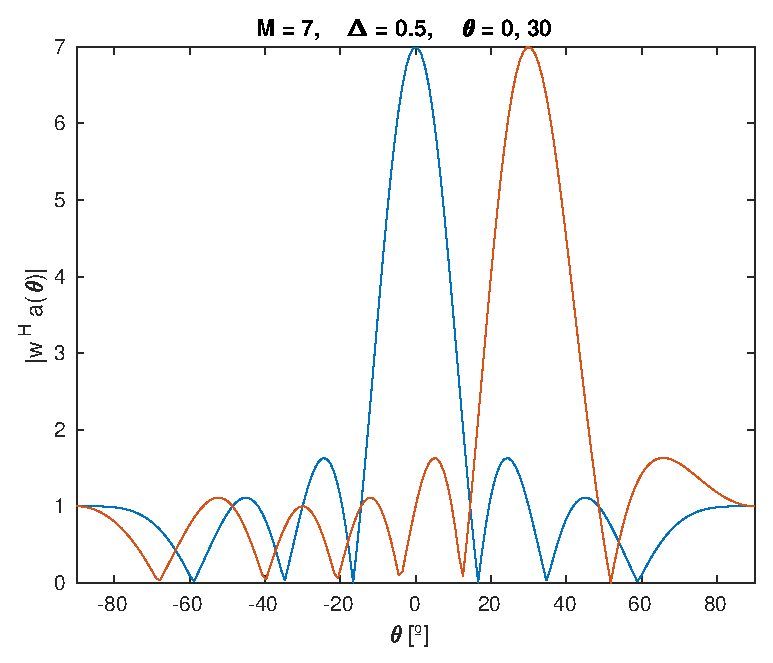
\includegraphics[width=.9\linewidth]{./assignment1/1.eps}
      \caption{A figure}
      \label{fig:test1}
    \end{minipage}
    \begin{minipage}{.49\textwidth}
      \centering
      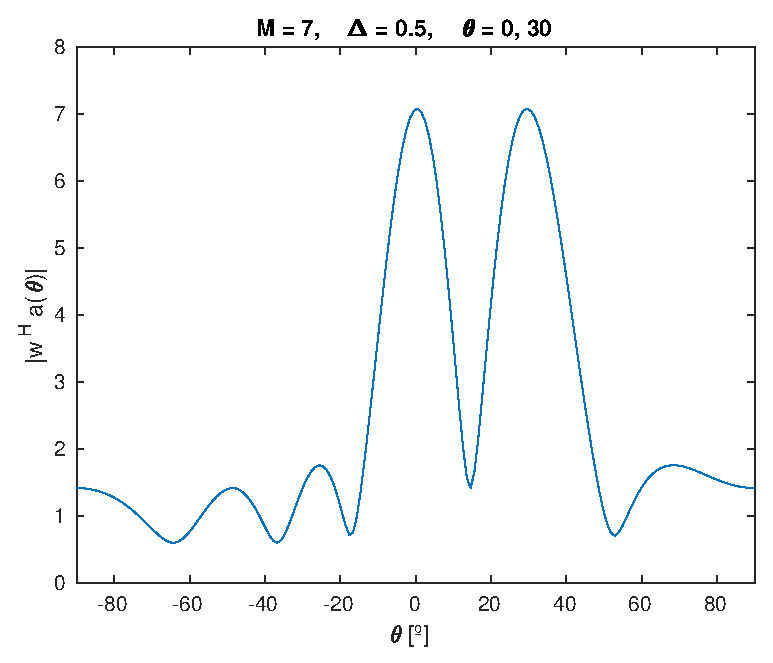
\includegraphics[width=.9\linewidth]{./assignment1/2.eps}
      \caption{Another figure}
      \label{fig:test2}
    \end{minipage}
\end{figure}

\par For figure \ref{fig:test1} I've applied one beamformer to a changing signal. The beamformers were exactly the same in structure, a matched filter, meaning $\mathbf{w} = \mathbf{a}(\theta)$, but one had $\theta = 0\degree$ and the other $\theta = 30\degree$ while the signal changed in directions, from -90 to 90 degrees.

\par This is NOT what you are suppose to do to estimate the spatial response of your beamformer. It is a way of knowing how much will you be able to take from the signal when it comes from all those directions but you are using a beamformer specific for one. In other words, that is evaluating a beamformer for a specific direction. But won't tell you how the principle of the beamformer performs faced with a signal that comes for more than 1 direction. 

Because we can change the signal very easily, by changing some parameters and generating a new set of data, we should rather check how will the beamformer perform in all directions if we are given a dataset that has signal coming from 2 directions.

In essence, it is the difference between checking what a specialized beamformer will take from the signal for signals coming from different directions if the beamformer is built for a certain $\theta$ versus how the beamformer will respond if crafted for different directions given that the signal comes from 2 in specific. Figure \ref{fig:test1} is the first case, Figure \ref{fig:test2} is the second case.


\vspace{.8cm}
\bb{Finally the truth}: neither case is what we are suppose to do, so why did I get the correct result?

When we did $\mathbf{w} = \mathbf{a}(\theta_1) + \mathbf{a}(\theta_2)$ and proceeded to change the source for different thetas, $\mathbf{a}(\theta)$, the response we were calculating was $y(\theta) = |\mathbf{a}(\theta_1)^\text{H} \mathbf{a}(\theta) + \mathbf{a}(\theta_2)^\text{H} \mathbf{a}(\theta)|$.

What we were suppose to do is check how would the matched filter receives the signal, thus, we should make $\mathbf{w} = \mathbf{a}(\theta)$ and the signal $x = \mathbf{a}(\theta_1) + \mathbf{w} = \mathbf{a}(\theta_2)$. Now, the response will be $y(\theta) = |\mathbf{a}(\theta)^\text{H} \mathbf{a}(\theta_1) + \mathbf{a}(\theta)^\text{H} \mathbf{a}(\theta_2)|$. 

Note that if we don't consider the absolute value of each response, they are the hermitian of each other. Considering the absolute value, the response will be the absolute (no pun intended) same! That was why the wrong thoughts resulted in the correct response. Luck, or bad luck, perspective dependent.

\vspace{.8cm}



\par The conclusions with the changes in the DOA, M, N and Delta is:
\begin{itemize}
    \item changing Delta affects only the ambiguity of our response as the array spatial response (a short transformation away for being the array radiation diagram) will be repeated more often. This will lead to wider lobes because only the non repetitive interval will be mapped into the array radiation diagram and if we plot the unambiguous interval of angles we see that the lobes will be wider.
    \item changing M influences the number of lobes. Them become more narrow as well because a bigger number of lobes must fit in the same unambiguous interval.
    \item varying N increases the resolution of the graph.
    \item The closer the two signals have Directions Of Arrival, the harder it will be to distinguish them and closer will be the maximum of the spatial responses. 
\end{itemize}

\par Finally, we were suppose to vary DOA, M, and the SNR to see changes in the singular values of X. First and foremost, we need to calculate and plot these values.

\par Singular Value Decomposition (SVD) is something that is very important. Again, remoting to other section: see  \ref{sec:important_mat_svd} and \ref{sec:important_math_spaces_relations} for a deeper svd insight and the explanation behind some conclusions.

\par There is a Matlab functions that calculates the SVD and the singular values will be in the diagonal of the central matrix. Plotting this values we see that:
\begin{itemize}
    \item decreasing the SNR will increase the singular values that should be 0;
    \item increasing the number of samples will increase all singular values because we'll have more contributions, simply to larger singular values, but the same singular vectors. That is why all singular values grow in the exact same proportion with N. It may help suppress the noise because threshold selection will be easier;
    \item the closer the DOA get, the more mixed with the noise will the singular values be. The second singular value will be closer to the noise;
    \item increasing M will increase only the singular values of interest because we'll be able to distinguish better the DOA and given them a bigger gain.
\end{itemize}

\par An important notion is that the more elements we have, the best directivity we can achieve paying by the increase in the number of secondary lobes. However, it will be far easier to distinguish directions. Actually, a formula that comes from Antenna Theory is that for a broadside array, where the main lobe is along the direction perpendicular to the orientation of the antenna elements: Main Beam Width = 2  arcsin $\frac{1}{M \bigtriangleup}$, where the $\bigtriangleup$ represents the distance in wavelengths between array elements.





\subsubsection{Convolutive Model}

\par Firstly, a pulse needs to be generated, the pulse to be transmitted. This can be done with a mathematical function of the pulse. 

\bb{function g = pulse(tau, L, P)}
\begin{itemize}
    \item \bb{tau} is the delay of the pulse. For tau = 0, the pulse should start in the beginning. For different delays, it should start later (there are no negative delays); 
    \item \bb{L} will be the channel length: there won't be considered any events passed L symbols from the present. In other words, the L-th symbol sent before the current one can still influence what is received. Before L, we don't consider the influence of any other symbol.
    \item \bb{P} will be the amount of samples taken in between symbols. This is a way of guaranteeing the correct reception because we'll create a much taller $\mathbf{X}$ matrix.
\end{itemize}

\vspace{.5cm}
\par The pulse function will be useful to construct the channel response. The channel response will be pulses scaled by each $\beta_i$ and delayed by each $\tau_i$, where $\beta_i$ and $\tau_i$ characterise the gain and delay of the path i from the sender to the receiver. Thus, the channel function will need these informations and will use the pulse function.
\par What it will do is add the pulses with the $\tau$ delays, $\beta$ scalings to a single signal which will be the channel. Each pulse required the channel taps length L to have enough zeros and P to sample the signal at those intervals.

\bb{function h = channel(tau, beta, L, P)}

\bb{One fulcral question to ask}: what if the inserted delays are not multiples of $\frac{1}{P}$? How will we do the pulses and thus the channel?
Well, because we are only interested in the sampling times, we will simply sample the signal at those instances. The delay will influence the value of that pulse at those sampling intervals and that should be accounted.

\vspace{.5cm}

\par As expected is necessary to create a signal to be transmitted. Changing the phase in quarters is enough to create a QPSK signal. This function returns N symbols of the source.

\bb{function s = source(N)}

\vspace{.5cm}




\par From the signal created, we must receive it. Thus passing it through the channel oversampled by a factor of P will create our complete vector of samples. It is important to note that is usual to separate the multipath effects (like we are experiencing here) from the spatial effects from having the signal coming from different directions. The macroscopic channel model is general enough to include both effects, we simply don't consider them at the same time for the simplicity of not working with matrices with more than 2 dimensions.

Indeed that is what happens, we've been calling the instantaneous model to the model where we don't oversample and don't consider multipath delays and calling convolutive model to the model where we do this yet only with one antenna.


\bb{function x = gen\_data1(h,s,P,N)}

This function creates a vector of convolutions: 
\begin{enumerate}
    \item Firstly, fills the source signal with P-1 zeros in between each symbol. This is a necessary step for the convolution with the channel;
    \item Then, convolves the resulting vector with the channel. This way, the channel is simulated and the oversampling as well.
\end{enumerate}

The result of this function is a vector of length $N\times P$. 
To create the matrix at the end, we need to reorganize this vector in columns of P elements.

\vspace{.5cm}

\par The final question was about the rank of the matrix A, with P rows and N columns. \uline{Well, the maximum rank is the smallest of the dimensions: if it has more unknowns than equations, the maximum rank is the number of equations. If it has more equations than unknowns, the maximum rank is the number of unknowns.}




%%%%%%%%%%%%%%%%%%%%%%%%%%%%%%%%%%%%%%%%%%%%%%%%%%%%%%%%%%
\subsection{Second Assignment}

\subsubsection{Receiver algorithms for the instantaneous Model}

As usual, we start with the instantaneous model, no time dependences. 
According to the data generation function previously built we are asked to implement a Matched filter, a Zero-forcing receiver and a Weiner Filter.
Note that contrary to the first assignment where the vector of weights was a vector, now it will be a matrix because we want to apply different vectors of weights to extract different directions of arrival of the signals. To apply receiver, one must only do the following:
\begin{equation}
    \mathbf{\hat{S}} = \mathbf{W}^\text{H} \mathbf{X}
\end{equation}

\par It is important know why they are different and in what they differ. After knowing that, simply by the way they act one can tell which type of receiver is implemented.



\bb{The Matched Filter} is nothing more than $\mathbf{W} = \mathbf{A}$. It minimises the noise by "turning the channel around". Because the channel has zero mean, it optimises the reception of the symbols with noise. $A^H (AS + N) = A^H AS + A^H N$.
It is a cheap receiver 
\todo{why?because is less computational intensive? cheap or just simple?}
Note however that the transpose of A normally is not its inverse (\uline{This would only be the case if the matrix was orthogonal} which doesn't happen in most situations). Thus this receiver is not expected to deliver the best results since it only addresses noise and disregards ISI.


\vspace{.5cm}
In a nutshell, the next receivers follow:

\quickimage{receivers.png}{.5}

The first refers to the Zero-forcing receiver, and is named like this because it tries to zero the difference between the received signal and the model, by changing A or S.

\bb{The Zero-forcing Receiver} in a line is: $\mathbf{W^H} = \mathbf{A}^\dagger = (\mathbf{A}^\text{H}\mathbf{A})^{-1} \mathbf{A}^\text{H}$, the pseudo-inverse of A. This, by definition, will invert A and thus nullify ISI.


\vspace{.5cm}

The second alludes to the Weiner Filter. Instead of minimising the difference between the received and estimated, it minimises the error between the estimated and the true symbols.

\bb{The Weiner Receiver}, also called the \ii{Linear Minimum Mean Square Error} (LMMSE) receiver, implements $\mathbf{w} = (\mathbf{AA}^\text{H} + \sigma^2 \mathbf{I})^{-1} \mathbf{A}$, a compromise between interference and noise, maximising the SINR.




\bb{Linearly Constrained Minimum Variance} LCMV, or \ii{Minimum Variance Distortionless Response} (MVDR) is practically a type of problem. We need to minimise something while constraint that some other thing hold. 
In particular, we want that $\mathbf{w}^H \mathbf{a} = 1$. Via the Lagrange Multipliers, we reach the answer: 
\begin{equation}
    \mathbf{w} = \mathbf{R}_x \mathbf{a} (\mathbf{a}^\text{H} \mathbf{R}_x^{-1}\mathbf{a})^{-1}
\end{equation}


The generalisation is as follows: 
\quickimage{mvdr.png}{.5}


This will be particularly important for the next part of the assignment.


%%%%%%%%%%%%%%%%%%%%
\subsubsection{Direction of Arrival Estimation}

This section shows how to apply the beamformers, but note that what we truly want is estimate the direction of arrival of the signal. Therefore, we will plot all the values instead of picking only the maximum.

With the standard beamformer, the direction of arrival can be found like:
\quickimage{doaestimation.png}{.5}

With the MVDR beamformer, the direction of arrival can be found this way:
\quickimage{doaestimation1.png}{.5}

With MUSIC, the direction of arrival is found following:
\quickimage{doaestimation2.png}{.5}


\par Then we just need to plot them in dB. By changing the number of elements in the array there is a gain in resolution. If we relax the proximity of the directions, to [0\degree,60\degree] for instance, there will be a very clear peak identified by each algorithm.


%%%%%%%%%%%%%%%%%%%%
\subsubsection{Receiver algorithms for convolutive model}
If we construct the Wiener Receiver for each Row of S\_L, we should take each column of H to do that!

Therefore, the beamformer would be:

\begin{equation}
    \mathbf{w} = (\mathbf{H}_i\mathbf{H}_i^\text{H} + \sigma^2 + \mathbf{I})^{-1} \mathbf{H}_i
\end{equation}

And the row we will be able to receive the best it he second one because the each column of H (remember H is P by L) has a symbol period, thus from where the most power is we can tell where the best response will be.  

Now, why do we take the columns of $\mathbf{H}$ as the beamformer for the rows of $S_L$? Simple, because that is what the beamformer does: it takes the columns of A to do exactly that. Note however that this beamformer uses the columns when estimating the symbol that came in direction d, using the a column to estimate a row. Thus, by analogy, we can use the same.

From the picture below, taken from the report submitted for this assignment, is possible to see that the most power is concentrated between the first and second symbol intervals:

\quickimage{report2h.png}{.6}







%%%%%%%%%%%%%%%%%%%%%%%%%%%%%%%%%%
\subsection{Third Assignment}
\par Similarly to the last part of the previous assignment, we should create a matrix of data with P rows and N columns, where along the rows are the samples between symbols and along a row are the symbols.

\subsubsection{Pilot-based Estimation}

\par Firstly, the previous function \bb{gen\_data1} now creates a vector of $M\times N$ samples where the noise is also included, this will be the received signal.


\par Then with that vector, knowing what is being transmitted, knowing as well what is being received, we should be able to extrapolate the channel.

\par Pilot-based Estimation is nothing more than estimation of the channel knowing what was transmitted.

From $\mathbf{X} = \mathbf{H S}$, we know that $\mathbf{H} = \mathbf{X S}^{-1}$, therefore we need to calculate the inverse of S. However, S is not a square matrix, thus we must do a pseudo-inverse! Matlab has a function to compute this pseudo-inverse and gives very accurate results. Depending on the SNR, the estimation will be more or less accurate.
Below the results of this estimation for two SNR values.


\begin{figure}[h]
    \centering
    \begin{minipage}{.49\textwidth}
      \centering
      \includegraphics[width=.9\linewidth]{./hw3/pilotEstimationSNR3.eps}
      \caption{Pilot estimation, SNR = 3dB}
      \label{fig:pilot1}
    \end{minipage}
    \begin{minipage}{.49\textwidth}
      \centering
      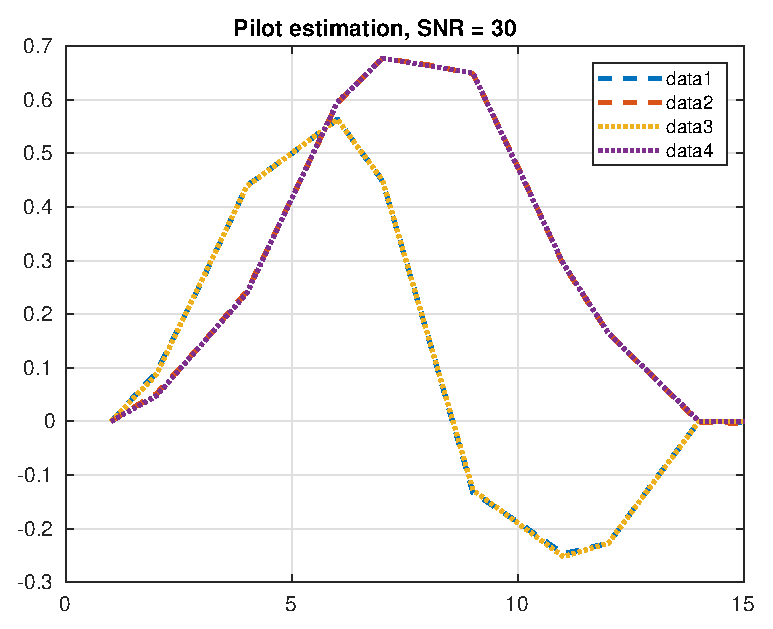
\includegraphics[width=.9\linewidth]{./hw3/pilotEstimationSNR30.eps}
      \caption{Pilot estimation, SNR = 30dB}
      \label{fig:pilot2}
    \end{minipage}
\end{figure}

The rest of the homework can have its own section

\section{Blind Estimation}

This is an important section. Without knowing what was transmitted or anything about the channel, just by knowing what was received, we may be able to extrapolate information from the channel. More precisely, from $\mathbf{X}$ we can tell if that is possible or not.

First, we compute SVD $()\mathbf{X})$ and get:

\quickimage{./hw3/fromslides1.png}{.5}

Recalling a slide:

\quickimage{./hw3/fromslides2.png}{.6}


And some important parts to take into account more carefully are that $\mathbf{\Sigma}_n$ is only non-zero in presence of noise.

This seems a weird way of writing the previous SVD formulation because what is now a sum was previously part of the same matrices, thus, how can them be summed together? Are them padded to have the same dimensions? Because zero padding matrices is ok as it doesn't change the space they span or anything like that.

Thus, the matrices with a subscript, like $\mathbf{U}_n$ and $\mathbf{V}^\text{H}_n$ will in fact have the same dimensions as the matrices obtained in the first SVD but with many more zeros. If the rank of $\mathbf{X}$ is r, then the matrices sizes will be:

\quickimage{./hw3/matSizePen.jpeg}{.2}


\uline{One important thing to notice} is that it is completely useless to add columns or rows of zeros. This may be the reason that sum is made in the slides without further justifications, because one can add them practically without notice because they don't change anything in the matrix.

With this said, one can more simply declare the matrices with subscripts:

\begin{multicols}{2}
    \begin{itemize}    
        \item $\mathbf{U}_s = \mathbf{\hat{U}}$
        \item $\mathbf{V}_s^\text{H} = \mathbf{\hat{V}}^\text{H}$
        \item $\mathbf{U}_n = \mathbf{\hat{U}}^\perp$
        \item $\mathbf{V}_n^\text{H} = \mathbf{\hat{V}}^{\text{H}\perp}$
    \end{itemize}
\end{multicols}


Now, from the relations presented in the slide above, we have matricial equations to find the channel or the symbols (depending the estimation we want to do). Because of the Toeplitz structure of H and S, we can massively simplify the problem. 

For Channel Estimation:
\quickimage{./hw3/blindChannel.png}{.5}


For Symbols Estimation:
\quickimage{./hw3/blindSymbols.png}{.5}


What both of these have in common in this clever construction is that we can gain many more equation than unknowns to make our problem solvable. Being solvable is having a solution or at least having a fundamental constraint not o have one. Lack of rank is not a fundamental constraint as with this organisation we can basically control the rank of the matrix we are multiplying to the channel or to the symbols. A fundamental constrain is when we can "add more rank" because increasing the number of rows that way won't add anything else ot the signal because the pattern is there already. 

So, it is very important to understand well what \uline{\bb{m}} is. \uline{m} will dictate the number of times we are going to repeat our original matrices in case of $\mathbf{V}_n$ or our original columns of $\mathbf{U}_s$. $\mathbf{U}_s$ will be m*P x (m*P-r) thus its transpose can always be divided in m sets of P columns.

Then, we need to calculate the row or columns nullspace of the resulting matrix to know if there is a unique and solution to our problem or if there are too many that we can't find the one we are looking for. This last part is related with the fundamental constraint.


So, after obtaining the matrices from the first SVD, we should build yet another matrix and choose an m that allows us to have full rank on the matrix we are looking for and then calculate the svd of that matrix and extrapolate if the problem is solvable or not. If it is, then the solution will be in the columns or rows nullspace of the matrix we just constructed. If that space and dimension 1, then we are a scalar away from the solution, meaning the symbols norm or angle needs to be scaled to "reality". That is not a big problem at all. However if we get a nullspace with dimension bigger than 2, it is already impossible to achieve the solution we are looking for.


\bb{Note} that the slides posted above, about channel and symbol estimation already say what subspace you should find: right nullspace for UnT, left nullspace for VnT. This because the Vn,T Matrix has a matrix on its left, while Un,T matrix has a matrix on its right. Thus the solution to those equations will be the nullspaces that when the matrix is used to multiply another at that nullspace side, it results in 0. AB=0 thus, solutions will lie in A right nullspace and B left nullspace.


% % % % % % % % % % % % % % % % % % % % % % % % % % % % % % % % % % % % % % % % %
\bb{The solutions of an homogeneous matricial equation lie in the left nullspace of the matrix on the right and on the right null space of the matrix on the left. If we decompose a matrix thought the SVD, U gives us the span of the columns but also the left nullspace,  the nullspace of the columns. These are orthogonal. And so are the span of the rows and the right nullspace, the nullspace of the rows. There is a relation between spans of columns(rows) and nullspaces of columns(rows), they are complementary: 
\begin{itemize}
    \item if the rank is smaller than the amount of columns, then the span of columns won't possible generate the full space, thus there will be a null space that complements the span, the left nullspace;
    \item if the rank is smaller than the number of rows, the span of the rows of the matrix can't possible have enough independent vectors to span the space of rows, and we call the right nullspace, nullspace of the rows or simply nullspace of the matrix to that subspace;
\end{itemize}
The left nullspace is the kernel of the matrix transposed and the nullspace simply the kernel of the matrix, by definition.
With this said, after calculating the SVD of the matrix constructed, one must check the dimensions of the correspondent nullspace. If the dimension is 1, then there can be found a solution. If there isn't, then there are way to many and the difference between them will practically always be more than a scalar.}
% % % % % % % % % % % % % % % % % % % % % % % % % % % % % % % % % % % % % % % % %

\uline{Important to notice as well is the m}: m is only the amount of time we will repeat the matrices. m is set by us as a mean of having an invertible H. We create a new, more exotic, calligraphic H that has the channel coefficients repeated in each row. Thus, we had M more equations and 1 unknown for each unit we increase m. This way, we will end up with a calligraphic H matrix that is $m \times M \times P$ by $L + m - 1$ and we just have to have an m sufficiently high that leads this matrix to be tall and thus invertible. This is where the conditions $m\ M \P \geq L + m - 1$ comes from. Further it simplifies to: $m \geq \frac{L-1}{MP-1}$.

This is very important because with $MP = 5$, we can only keep an $m = 1$ until the L reaches 5. However, increase the channel can bring other problems besides invertibility, even if it is only increased with zeros\dots


%%%%%%%%%%%%%%%%%%%%%%%%%%%%%%%%%%%%%%%%%%%%%%%%%%%%%%%%%%%%%%%%%%%%%%%%%%%%%%%%%
\section{Final Assignment}

\subsection{Estimation of Directions and Frequencies}

\subsubsection{Signal Model}
The data generation is basically:
\begin{itemize}
    \item using gen\_a for generating the steering vectors, i.e matrix A, for the directions of arrival;
    \item generating the signal as described. It has always unitary energy by the assignment, thus the power will be unitary and we won't need to go through what we've done to get the signal power to know the variance of the noise to apply;
    \item Despite source energy is 1, and the elements of A having modulus 1, the signal A*S doesn't have power 1. Thus, we need to use that power to compute the SNR and find the variance of the noise to be added to the signal to achieve the required SNR.
\end{itemize}

\par Then, as a good practice, we should plot the singular values and see if the expected variations are taking place.

\subsubsection{Estimation of directions}
\bb{ESPRIT} is the best way of estimation directions of arrival of the signals. It doesn't need to sweep the entire space of directions.

\par The method is very well outlined in the slides. 
\begin{enumerate}
    \item We need a signal with a certain structure of its column space. Because its column space is a subset of the space spanned by A, in case of $X = AS$, then A needs to have a specific structure. That structure is shift-invariance: the element below should always be a factor away from the above.
    
    \quickimage{esprit1.png}{.5}

    This is important because this property is a space assumption that if met can simplify the computations tremendously.

    \item We need to start grouping from the matrix X as we did in the above example. The matrix X is M by N, sensors by samples, and will be divided in a new X and a Y:
    
    \quickimage{esprit2.png}{.5}

    \par This new X and Y construct, from taking all but the last and all but the first rows of the received samples vector, respectively. They can be obtained in a different way, but that is what we are trying to estimate!
    \bb{Note:}our objective will be the matrix $\Theta$ with the $\phi$. From those entrances in the diagonal we invert the to retrieve the thetas.

    \item Stack them: \quickimage{esprit3.png}{.5}
    \item Compute the SVD of $\mathbf{Z}$. \bb{HOWEVER:} Bear in mind that what we really want in the economy size svd. Because of noise that won't be possible, thus we have to take from U the parts that matter to get the signal that interests us.
    \begin{equation}
        \mathbf{Z} = \mathbf{\hat{U}}_z \mathbf{\hat{\Sigma}}_z \mathbf{\hat{V}}^\text{H}_z
    \end{equation}

    \par The dimensions of Z should be: 2 $\times$ (M-1) by N.
    \par Thus, $\mathbf{\hat{U}}_z$ should be 2 $\times$ (M-1) 
\end{enumerate}


Note that ESPRIT can estimate very effectively and efficiently a vector with the structure of a steering vector, i.e the next element can be obtained from the previous by a multiplication from a $\phi$. ESPRIT returns that $\phi$. Thus, one may do the same for the transmitted symbols because they depend on the frequency. One can do the same to delays because they can be represented in the frequency domain by a phase shift. And one can even find the frequencies of signals which the symbols don't depend that directly on frequency, but knowing that each signal can be decomposed in a Fourier Series with many frequencies which will be represented as exponentials in time.


\subsubsection{Estimation of frequencies}
In particular, for this frequency estimation one simply had to note the similarities between the two problems.

If $\mathbf{X} = \mathbf{AS}$, allows the complete $\theta$ estimation from A given X, then $\mathbf{X}^T = \mathbf{S}^T\mathbf{A}^T$ should allow the complete frequency estimation, given that we provide the algorithm with X transposed.

This not only will put the symbols in a column, achieving the structure we need, but will make X transposed have its range as a subspace of the span of the columns of $S^T$, thus making the estimation possible. Because we are going to estimate the factor that relates consecutive elements, we then need to get the frequencies out.


\subsubsection{Comparison}
From the previous derived ESPRIT implementations for estimating frequencies and DOA, we can construct the matrices S and A, respectively.
From there, knowing $\sigma$ of the noise, one may create the ZF beamformers.

One of them will perform better than the other, but why?

The answer lies in what we are estimating. From the esprit for thetas, we estimate the thetas based on the columns of A, which are are determined exactly and span the subspace of columns of X. On the other hand, determining S will make us able to estimate A instead of determining it precisely, thus resulting in worse results in terms of interference.


\subsubsection{Constant Modulus Algorithm}
After the implementation, in accordance with the respective section in this document one will notice:
\begin{itemize}
    \item the resultant beamformer will depend on $\mathbf{w}_{init}$, on $\mu$ (the step size) and on the number of samples
    \item Depends on the number of samples because it needs enough iterations to converge the estimations into modulus 1; The amount of samples it takes to converge depends also on the step size: it converges faster for a bigger step size. However, it may not converge if the step size is too big;
    \item 
\end{itemize}







%%%%%%%%%%%%%%%%%%%%%%%%%%%%%%%%%%%%%%%%%%%
\section{Extra Slides}

\subsection{Channel Estimation and Hybrid Precoding for mmWaves}
Millimeter Waves need beamforming or else the additional attenuation wouldn't make the communication worth the higher frequencies and probably even worse than many other solutions that we've right now.

To do beamforming, we need an array of antennas, the more the better. And ideally, an array of radiofrequency chains coming directly from the the baseband processing that is done para a computer. However, this is tremendously expensive. What's done instead is using less radiofrequency chains with pre-defined precoders, like phase shifters. But one can't use just one RF chain and a lot of phase shifters because that would take away all the flexibility. An hybrid approach requires a new set of estimation algorithms to account these phase shifters and play with them to estimate and optimise the channel utilization.

\subsection{UltraSound}
There a tradeoff between frequency (or SNR) and resolution. Higher frequencies penetrate worse but provide a better resolution due to their smaller wavelength, one can better distinguish different scatterers. This is why  resolution gets worse the deeper we try to see.






\section{Evaluation}

\subsection{Relation of single values after sensors or samples change}

Knowing that the sensors double or that the amount of samples double, what will be the effect on the single values? One my know!
Changing the amount of sensors increases the size of the H matrix, increasing the number of samples increases the size of the S matrix. None of the sizes matters for the multiplication. Therefore, doubling either one will simply double the size of X.

How does doubling the size of X affects X Frobenius Norm? Know that the formula is given by: $\sum_{i,j} |x_{ij}|^2$, by increasing one of the sizes we simply double the size of X thus, multiplying that sum by 2. X can be decomposed in singular values and the norm of those matrices will be the norm of the central matrix because the other two are unitary, thus have norm one and the norm of the total is the multiplication of the norm of each one.

In this case, because we are increasing the dimensions by 2, the sum of the squares along the diagonal which is the Frobenius Norm of the matrix will have double the elements, thus the sum is doubled. Considering that they are equal (and there are 3 of them): \\
$3 \sigma_{new}^2 = ||X_{new}||_F^2 = 2 ||X_{old}||_F^2 = 2 \cdot 3 \sigma_{old}^2 \Leftrightarrow \sigma_{new} = \sqrt{2} \sigma_{old}$


\subsection{Wiener and ZF receivers}

The next question was about the Weiner and ZF receivers. By remembering what equations each one is trying to minimise, one can deduce them. By knowing S, knowing that the ZF attempts to minimise $||X - \hat{A}S||$, then $\hat{A} = X S^\dagger$. And thus, the beamformer is $W^\text{H} = A^\dagger = (XS^\dagger)^dagger$.

Note that this is very different than the beamformer presented $W^H = S X^\dagger$. This beamformer comes from the minimisation of $||W^HX - S||$, thus being a Wiener Receiver. 

\subsection{Blind Estimation deduction and nullspaces relations}

The last and the question I performed the worse was the one where a deduction for Blind Estimation was necessary.

For the symbols, $V_n$ has the nullspace along its columns. As $V_n^\text{H}$ is N-1 by N-1-(r)  where r is the number of singular values due to noise, zero in its absence.

So, for the matrices to match, and because $V_n^\text{H}$ has the row nullspace along its rows (the rightnullspace), $V_n^H X^H = 0 \Leftrightarrow X V_n = 0$.

\uline{Don't forget how to multiply things to obtain zero from the nullspaces}

This makes sense because: the rows of $V_n^\text{H}$ have the nullspace of rows of X, thus these rows need to by multiplied to the rows of X to get 0, therefore is needed to user X transposed (remember that rows of the left matrix multiply to columns of the right one). Likewise, when he transpose to $V_n$, now we have the nullspace along the columns. Then this matrix needs to be on the right to originate something that is a linear combination of the columns. By having the rows of X make this product, having X on the left, the "interception" will occur and because they are orthogonal, give 0.


\end{document}
 











 